
\documentclass[journal,  onecolumn, 12pt]{IEEEtran}

\usepackage{setspace}
\usepackage{amsfonts}
\usepackage{textcomp}
\usepackage{microtype}
\usepackage{algorithm}
\usepackage{graphicx}
\usepackage{wrapfig}
\usepackage[noend]{algpseudocode}
\usepackage{commath}
\usepackage{booktabs}
\usepackage{bm}
\usepackage{amssymb}
\usepackage{cite}
\usepackage{amsmath}
%\usepackage{algorithmic}


\begin{document}

\title{Noise Processing in Automatic Speech Systems: A survey}


\author{Soumi Maiti \\The Graduate Center, CUNY}
\maketitle

\begin{abstract}

\end{abstract}











\section{Introduction}
\section{Noise in Speech}
As we live in a noisy environment, when speech is recorded some amount of noises are always added. Humans are habituated with some amount of noise and they can process speech with noises at least in a little amount. With large amount of noise humans have difficulty with proper hearing. In speech systems this difficulty is larger and more prominent. Depending on the statistical relationship of noise and the signal noise in speech systems can be classified into two categories: \emph{correlated noise} and \emph{uncorrelated noise}. 

\paragraph*{Correlated Noise}
Noise can be correlated with speech signal. Some example of such noises are reverberation, echo etc. Reverberation is prolongation of a sound or resonance. It occurs when sound source is present in a closed space, like in a room or hall. As sound strikes a wall, some of it is reflected while some of the sound is absorbed by the wall. Some of the absorbed signal can produce heat and some of it is transmitted through the wall. The amount of deflection and absorption is depended on the quality and position of the wall. In a closed space sound gets deflected multiple times and and we can hear it as a resonance. Echo occurs when reflected sound reaches to the listener separately from the original sound. Echo occurs in bottom of the walls, by buildings, by an empty room. These two type of noises are generally present with sound unless sound source is in a anechoic room which absorbs all sound. 

\paragraph*{Uncorrelated Noise}
Uncorrelated noise are not generated from sound at all. All kinds of environmental sounds gets added with speech naturally. If one or more persons are speaking in the background that is treated as speech noise. Noises in road like car noise or bus noise are also another example of environmental noises. If there is music playing in the background it can also be treated as noise.

There are other possible classifications, for example based on power spectral density, i.e. colored noise.

The study of noise in automatic speech recognition systems is critical. As discussed in \cite{Lippmann1997Speech}, the performance of machine based speech recognition systems are greatly affected by noise, much more than human listeners.

\subsection{Humans versus Machine}
In presence of noise performance of speech recognizers degrades rapidly. This effect was first observed in \cite{Lippmann1997Speech} when the author compared human listeners with speech recognizers through varying type of speech. Performance of ASR is lower than humans. When they add the speech with car noises and repeat the experiment. With little noise there is no degradation in human listeners,even with high noise performance degrades slightly. With ASR even with little noise the performance worsens. ASR error rate reaches to almost 100\% at SNR 0dB. It is difficult for ASR to recognize any noise that it hasn't seen before. To compensate that, the authors train the recognizer with car noise. Even with this noise adaptation error in ASR is more than 40\% of the quieter case. They also compare performance of ASR to humans in a office room environment. Similar performance degradation in presence of noise is seen. 
\begin{wrapfigure}{L}{0.5\textwidth}
\centering
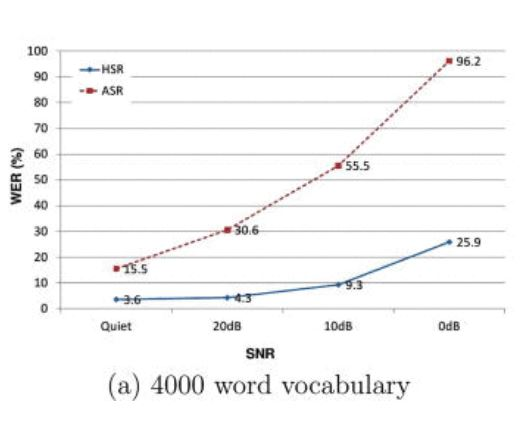
\includegraphics[width=0.45\textwidth]{Juneja}
\caption{ASR vs. human listener with 4000 words vocabulary with correlated noise}
\label{fig:jun}
\end{wrapfigure}
Speech recognizers has seen huge improvement in their performance in recent years. Juneja at el. \cite{Juneja2012} compares the performance of ASR and humans again in 2012(Fig \ref{fig:jun}). He observes that though ASR performance has improved in quieter case, in presence of noise performance degradation is still very high reaching almost 96\% at SNR less than 0 dB.  



\paragraph*{Practical Impacts} The presence of noise causes performance degradation in many applications such as:
\begin{itemize}
\item Automatic speech recognizers: An increase in recognition error as reported in \cite{Lippmann1997Speech,Juneja2012,Scharenborg2007}.
\item Hearing Aid: Increases speech reception threshold as shown in \cite{FestenAndPlomp1990,Kochkin2012}.
\item Cochlear implants: More power hungry systems required to maintain signal quality \cite{FriesenEtAl2001}.
\item Telecommunication systems: Degradation in the quality of the received signal \cite{Hecht2014,SmithAndPage2015}.
\end{itemize}

\paragraph*{Quantifying the effects}

\begin{wrapfigure}{L}{0.5\textwidth}
\centering
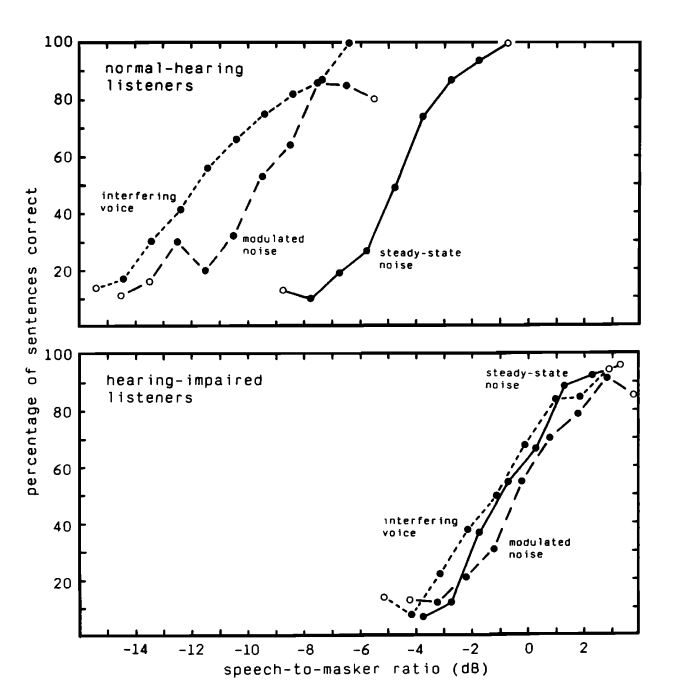
\includegraphics[width=0.45\textwidth]{Cocktail.JPG}
\caption{Normal hearing (left) vs. hearing impaired (right)}
\label{fig:noise}
\end{wrapfigure}

Festen et al\cite{FestenAndPlomp1990} compared performance of hearing impaired listeners and normal hearing listeners with different mix of noises. He used steady state noise, modulated noise and interfering speech as background noise. In humans effect of different noises were different. Normal hearing listeners are less effected by interfering speech, not observed with hearing impaired(Fig. \ref{fig:noise}). 

\subsection{Cocktail Party Problem}
Humans are generally good at focusing auditory attention even when other noises are present in background. For example humans are able to continue conversation in a noisy room. Imagine a cocktail party where many groups are talking simultaneously. Humans are able able to communicate in cocktail parties \cite{bronkhorst2000cocktail,pollack1957cocktail,arons1992review,hawley2004benefit}. Sometimes to compensate with loud noise in background we speak loudly, this effect is known as Lombard Effect. With speech recognizers it is very difficult. The signal is a speech signal but so is the noise! Recognizers cannot separate signal from noise. 

\paragraph*{TODO: Simplification}
For machines it is difficult to separate speech with speech mixtures when multiple people are speaking in the background. With some constraints and simplified problem, it is possible to recognize speech. \cite{TuEtAl2014,WengEtAl2015} models only two people speaker, one being louder and another being quieter. Hershey et al \cite{HersheyEtAl2010} models a known set of speakers and two speaker mix. He uses graphical modeling with acoustic and grammar information to model each speaker. Then using this model, first recognize two speaker in the mix and use this information to separate signal and recognize speech. 



\section{Metric of Quality}

\section{Noise Removal Algorithms}

\section{Speech Synthesis}

%\begin{figure}[!t]
%\centering
%\includegraphics[width=2.5in]{myfigure}
% where an .eps filename suffix will be assumed under latex, 
% and a .pdf suffix will be assumed for pdflatex; or what has been declared
% via \DeclareGraphicsExtensions.
%\caption{Simulation results for the network.}
%\label{fig_sim}
%\end{figure}

%\begin{figure*}[!t]
%\centering
%\subfloat[Case I]{\includegraphics[width=2.5in]{box}%
%\label{fig_first_case}}
%\hfil
%\subfloat[Case II]{\includegraphics[width=2.5in]{box}%
%\label{fig_second_case}}
%\caption{Simulation results for the network.}
%\label{fig_sim}
%\end{figure*}
%

%\begin{table}[!t]
%% increase table row spacing, adjust to taste
%\renewcommand{\arraystretch}{1.3}
% if using array.sty, it might be a good idea to tweak the value of
% \extrarowheight as needed to properly center the text within the cells
%\caption{An Example of a Table}
%\label{table_example}
%\centering
%% Some packages, such as MDW tools, offer better commands for making tables
%% than the plain LaTeX2e tabular which is used here.
%\begin{tabular}{|c||c|}
%\hline
%One & Two\\
%\hline
%Three & Four\\
%\hline
%\end{tabular}
%\end{table}


\newpage
\bibliographystyle{plain}
\bibliography{ref}

\end{document}


